\documentclass[a4paper,10pt]{article}
\usepackage[utf8]{inputenc}
\usepackage{graphicx}
%opening
\title{Offensive Security\\Lab-report 4}
\author{Moritz Rupp}

\begin{document}

\maketitle

\begin{abstract}

\end{abstract}
\newpage
\section{Lab 4}
\subsection{A Basic Stack Overflow Attack}
We are provided with a vulnareble piece of C Code that can be exploited to trigger a basic Stack overflow. Since modern architectures have several countermeasures to prevent such abuse, we have to compile the Code as shown in the lecture nodes to deactivate them!
\begin{center}
 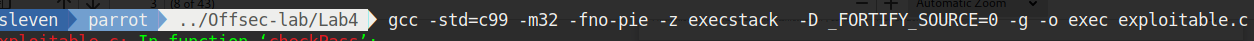
\includegraphics[scale=0.3]{gcc.png}
\end{center} 
After failing to trigger the exploit by passing different input lengths, we take a closer look at the programm with the help of GDB.\\
At first we look at the assemler Code. To make it more readable we set the disassembler flavor to intel. 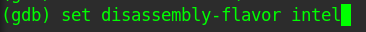
\includegraphics[scale=0.4]{intelfalvor.png}\\
After further inspection we realize that we need to find the starting adress of the hidden function, that includes the 'Flag' that proves the success of the attack.
\begin{center}
 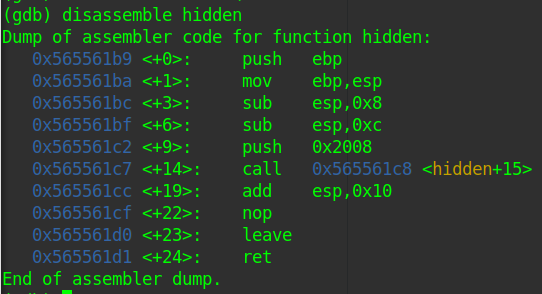
\includegraphics[scale=0.5]{hidden.png}
\end{center}
Starting adress is '0x565561b9'.\\
When we pass this adress as the 'overflow' we can execute the function 'hidden'.

\end{document}
